\label{tag:experiment}
本研究ではLTIを用いることで実際に複数のLMSから、独立したWebアプリケーションであるネットワーク自己学習機能を同じように学習支援ツールとして呼び出すことができるのかを確認するために、LTIに準拠したLMSであるMoodle、Canvasを用いての実装実験を行った。\\

\subsection{LTI使用方法}
LMS上でTool Provider(ツール・プロバイダ)を使用するには、各LMS上で外部ツールの設定を変更する必要がある。例として、moodleでの使用方法を説明する。\\
moodleでは外部ツール設定より図\ref{fig:moodle config}参照、ツール名、ツールURL、コンシューマキー、秘密鍵の設定をする必要がある。これらの設定を得て、moodleからTool Provider(ツール・プロパイダ)を利用することが可能となる。\\
\begin{figure}[htbp]
  \begin{center}
    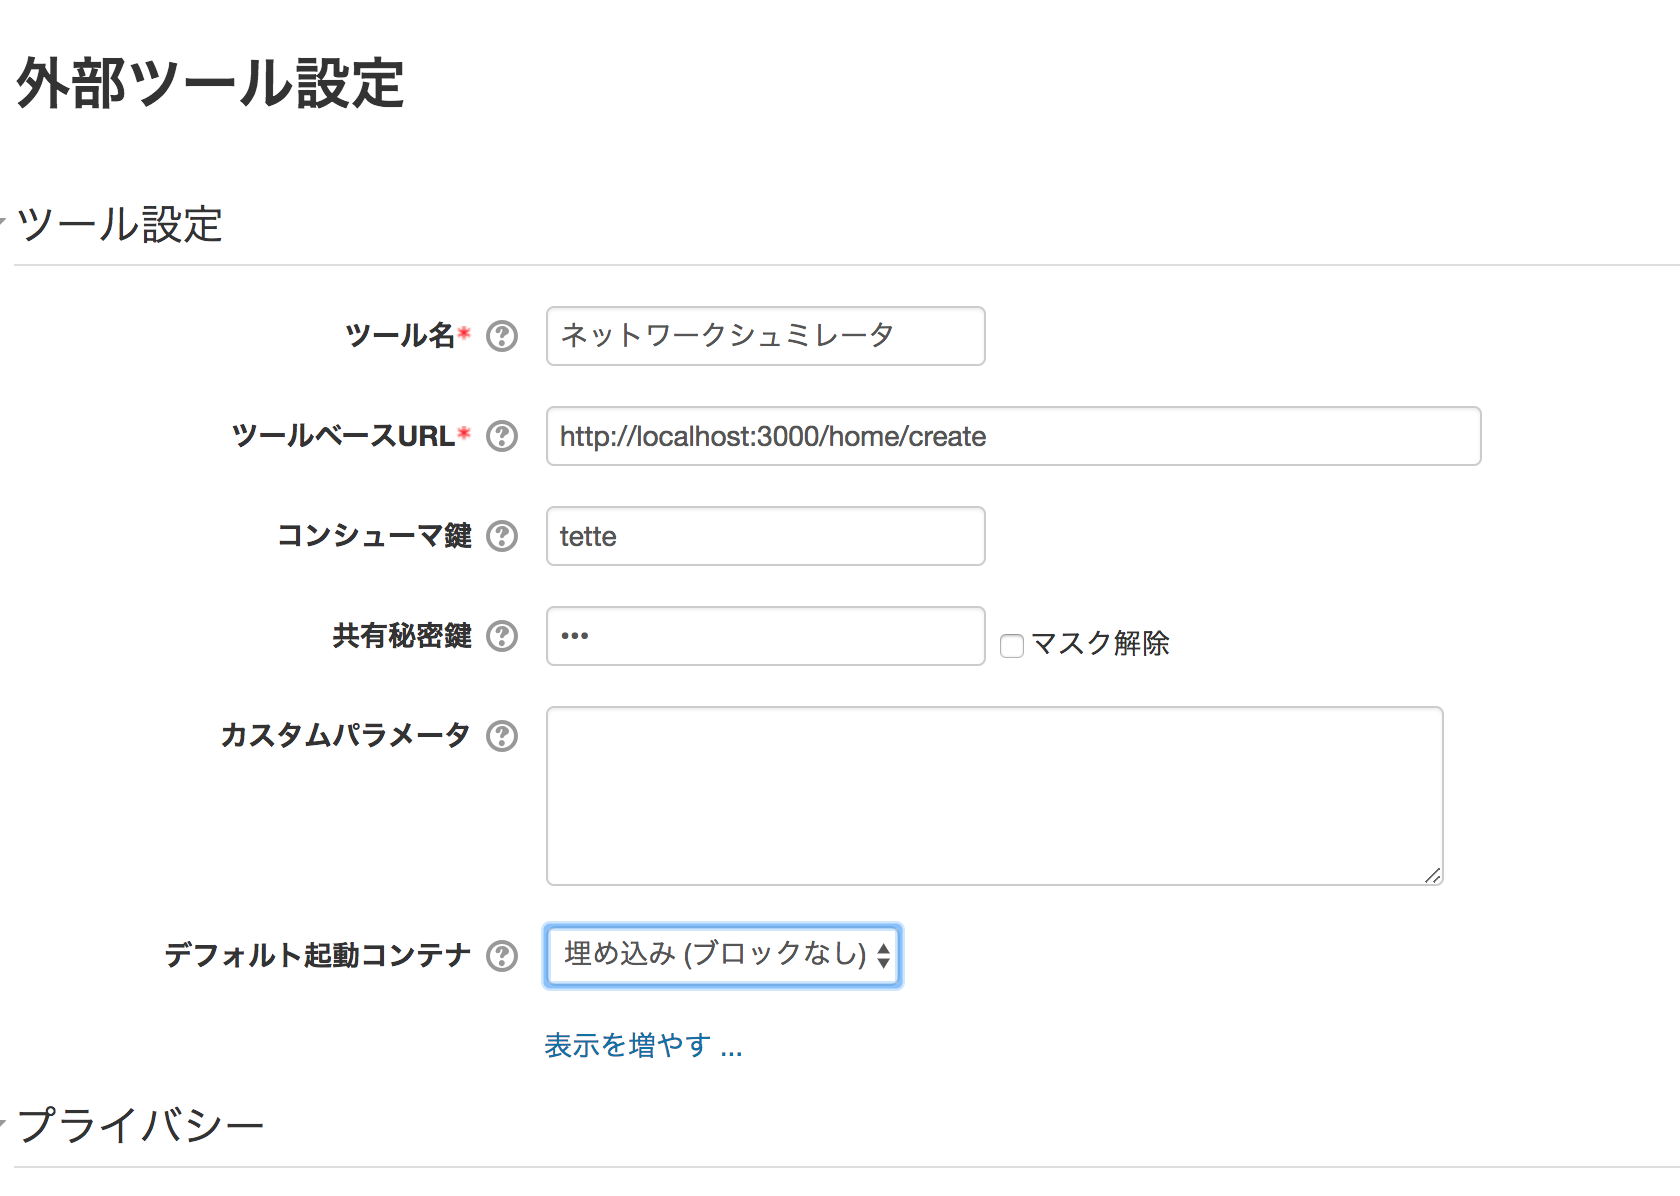
\includegraphics[clip,width=12.0cm,height=8.0cm]{img/moodleSet.png}
    \caption{moodle 外部ツール設定画面}
    \label{fig:moodle config}
  \end{center}
\end{figure}

\subsection{成績反映}
Moodleにおいて、実際に成績反映できるかどうかの実験を行った結果をいかにしめす。
